\section{Methods}
\label{sec:data}

\textbf{Simulations:} In order to compare the two methods while controlling for their correct performance, we simulated a 400 seconds (TR = 2 s) activity-inducing signal with five neuronal events, convolved it with the canonical HRF, and we added noise of different sources (physiological, thermal, and motion-related) with different signal-to-noise ratios (SNR = [20 dB, 10 dB, 3 dB]) that represent low, medium and high levels of noise as shown in Figure~\ref{fig:simulations}.

\begin{figure}[h]
    \begin{center}
        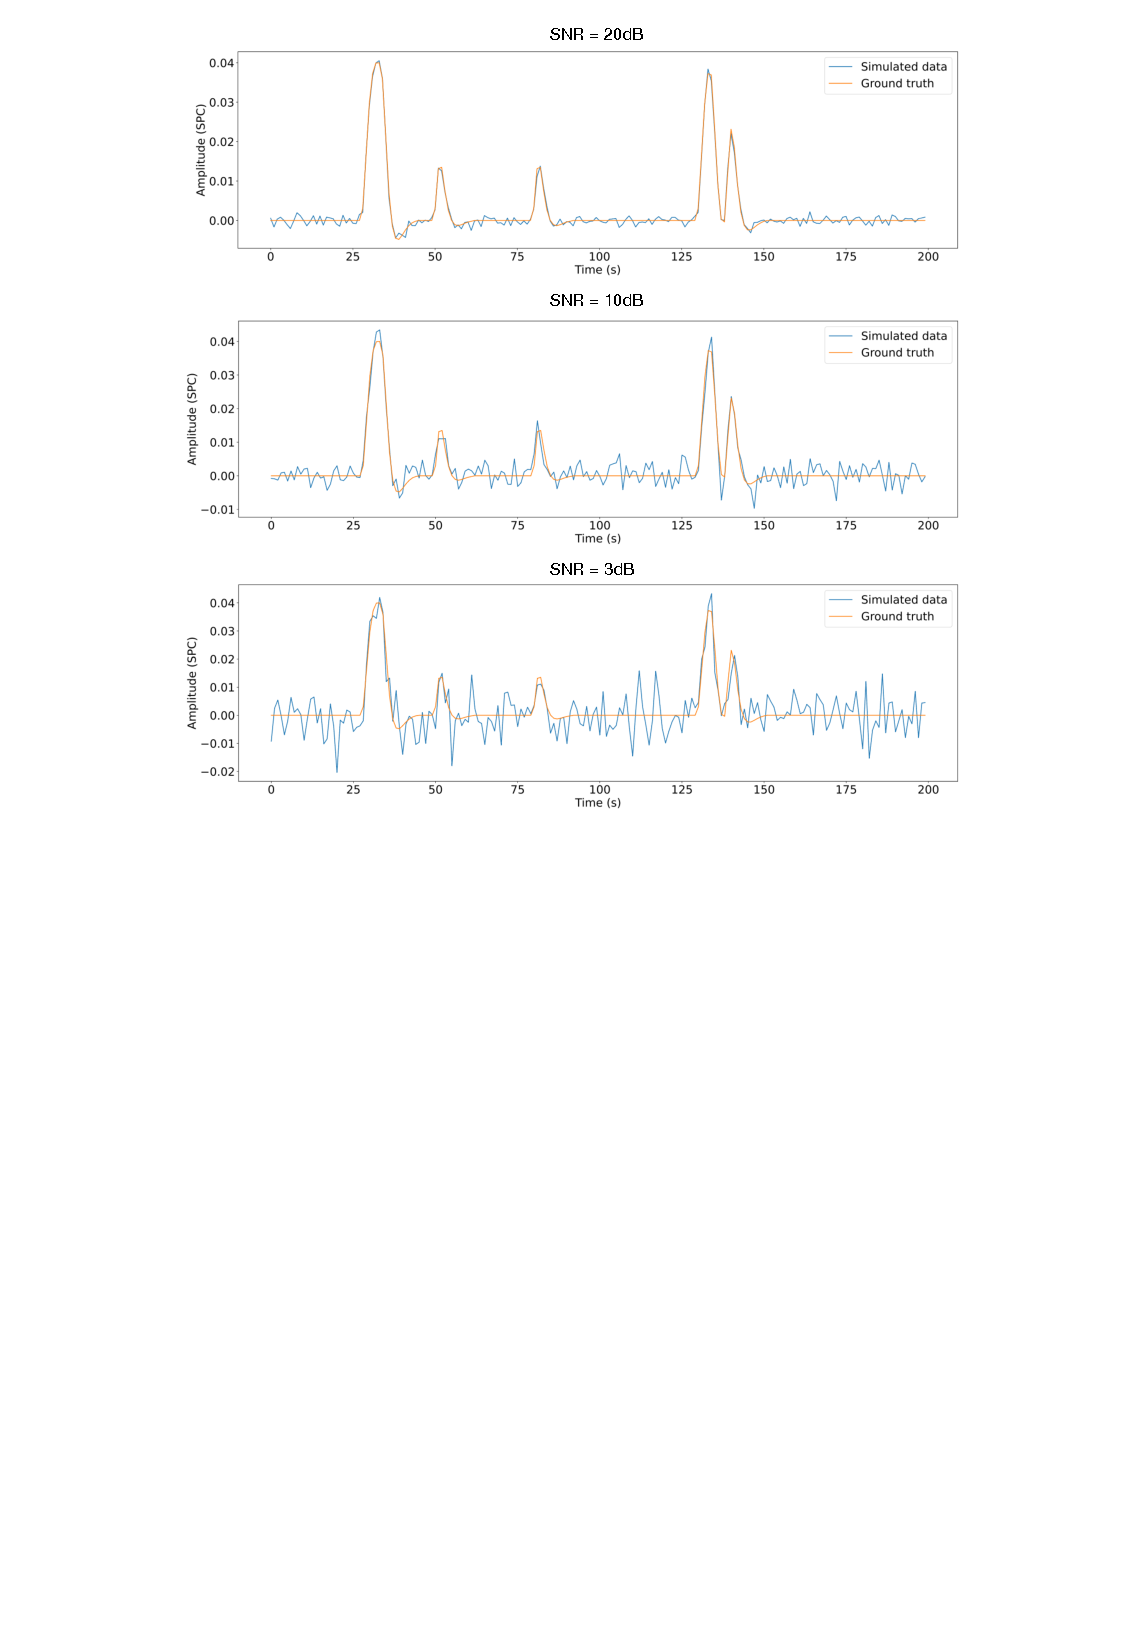
\includegraphics[width=\columnwidth]{figures/sim.pdf}
    \end{center}
    \caption{Simulated signal with different SNRs (20 dB, 10 dB and 3 dB).}
\label{fig:simulations}
\end{figure}

\textbf{Motor task dataset:} One healthy subject was scanned in a 3T MR scanner (Siemens) as part of a larger experiment under a Basque Center on Cognition, Brain and Language Review Board-approved protocol. T2*-weighted multi-echo fMRI data was acquired with a multiband (MB) multi-echo gradient echo-planar imaging sequence (340 scans, 52 slices, Partial-Fourier = 6/8, voxel size = 2.4x2.4x3 mm\textsuperscript{3}, TR = 1.5 s, TEs = 10.6/28.69/46.78/64.87/82.96 ms, multiband factor = 4, flip angle = 70\(^o\), GRAPPA = 2).

During the fMRI acquisition, subjects performed a motor task consisting of five different movements (left-hand finger tapping, right-hand finger tapping, moving the left toes, moving the right toes and moving the tongue). These conditions were randomly intermixed every 16 seconds, and were only repeated once the entire set of stimuli were presented. Data preprocessing consisted of optimally combining the echo time datasets, detrending of up to 5\(^{th}\)-order Legendre polynomials, spatial smoothing (3 mm FWHM) and normalization to signal percentage change. For this comparison, we selected a voxel that best represented the right-hand finger-tapping paradigm based on a generalized linear model as shown in Figure~\ref{fig:finger_tapping}.

\begin{figure}[h]
    \begin{center}
        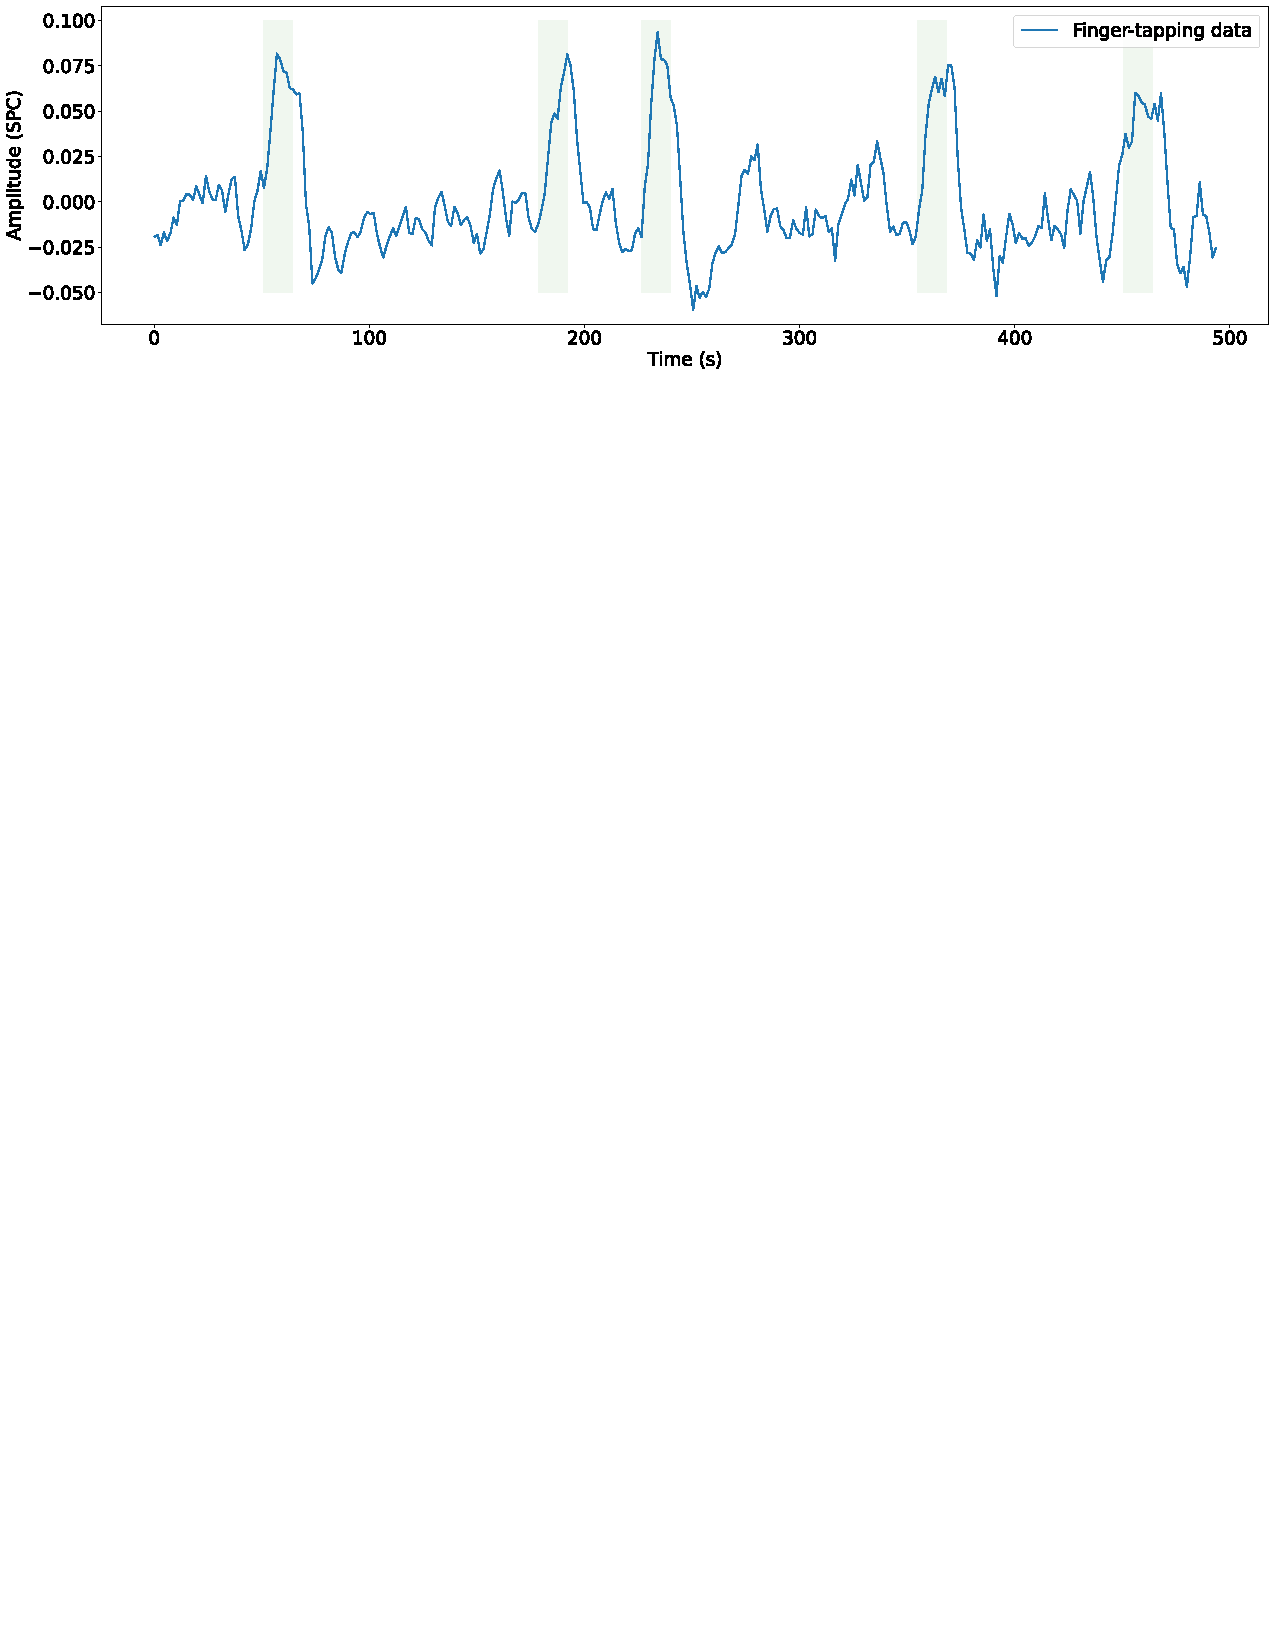
\includegraphics[width=\columnwidth]{figures/finger_tapping.pdf}
    \end{center}
    \caption{Most representative voxel of the finger-tapping task. Green blocks indicate the onsets and the duration of it.}
\label{fig:finger_tapping}
\end{figure}

\textbf{Resting-state datasets:} One healthy subject was scanned in a 3T MR scanner (Siemens) as part of a larger experiment under a Basque Center on Cognition, Brain and Language Review Board-approved protocol. Two runs of T2*-weighted fMRI data were acquired during resting-state, each with 10 min duration, with 1) a standard gradient-echo echo-planar imaging sequence (monoband) (TR = 2000 ms, TE = 29 ms, flip-angle = 78\(^o\), matrix size = 64x64, voxel size = 3x3x3 mm\textsuperscript{3}, 33 axial slices with interleaved acquisition, slice gap = 0.6 mm) and 2) a simultaneous multislice gradient-echo echo-planar imaging sequence (multiband factor = 3) developed by the Center of Magnetic Resonance Research (University of Minnesota, USA; TR = 800 ms, TE = 29 ms, flip-angle = 60\(^o\), matrix size = 64×64, voxel size = 3x3x3 mm\textsuperscript{3}, 42 axial slices with interleaved acquisition, no slice gap). Single-band reference images were also collected in both resting-state acquisitions for head motion realignment.

During both acquisitions, participants were instructed to keep their eyes open, fixating a white cross that they saw through a mirror located on the head coil, and not to think about anything specific. Field maps were also obtained to correct for field distortions.